\documentclass[a4paper,12pt]{article}
\usepackage[slovene]{babel}
\usepackage[utf8]{inputenc}
\usepackage{graphicx}
\usepackage[T1]{fontenc}
\usepackage{lmodern}
\usepackage{url}
\usepackage{cite}
\usepackage{amsthm}
\usepackage{amssymb}
\usepackage{listings} %za pisanje kode
\usepackage{float} %za natančno specificiranje pozicije slik
\usepackage[a-1b]{pdfx}

\lstset{basicstyle=\small\ttfamily,xleftmargin=\parindent}
\usepackage{tikz}

\textwidth 15cm
\textheight 24cm
\oddsidemargin.5cm
\evensidemargin.5cm
\topmargin-5mm
\addtolength{\footskip}{10pt}
\pagestyle{plain}
\overfullrule=15pt

% ukazi za matematicna okolja
\theoremstyle{definition} % tekst napisan pokoncno
\newtheorem{definicija}{Definicija}[section]
\newtheorem{primer}[definicija]{Primer}
\newtheorem{opomba}[definicija]{Opomba}

\renewcommand\endprimer{\hfill$\diamondsuit$}

\tikzset{
  treenode/.style = {shape=rectangle, rounded corners,
                     draw, align=center,
                     top color=white, bottom color=white!20},
  env/.style      = {treenode, font=\ttfamily\normalsize},
  dummy/.style    = {circle,draw}
}

% ukaz za slovarsko geslo
\newlength{\odstavek}
\setlength{\odstavek}{\parindent}
\newcommand{\geslo}[2]{\noindent\textbf{#1}\hspace*{3mm}\hangindent=\parindent\hangafter=1 #2}

\newcommand{\program}{Finančna matematika} % ime studijskega programa: Matematika/Finan"cna matematika
\newcommand{\imeavtorja}{Ana Golob} % ime avtorja
\newcommand{\imementorja}{prof. dr. Andrej Bauer} % akademski naziv in ime mentorja
\newcommand{\naslovdela}{Prestrezniki in algebrajski učinki  na primerih iz finančne matematike}
\newcommand{\letnica}{2018} %letnica diplome

%%%%%%%%%%%%%%%%%%%%%%%%%%%%%%%%%%%%%%%%%%%%%%%%%%%%%%%%%%%%%

\begin{document}

% od tod do povzetka ne spreminjaj nicesar
\thispagestyle{empty}
\noindent{\large
UNIVERZA V LJUBLJANI\\[1mm]
FAKULTETA ZA MATEMATIKO IN FIZIKO\\[5mm]
\program\ -- 1.~stopnja}
\vfill

\begin{center}{\large
\imeavtorja\\[2mm]
{\bf \naslovdela}\\[10mm]
Delo diplomskega seminarja\\[1cm]
Mentor: \imementorja}
\end{center}
\vfill

\noindent{\large
Ljubljana, \letnica}
\pagebreak

\thispagestyle{empty}
\tableofcontents
\pagebreak

\thispagestyle{empty}
\begin{center}
{\bf \naslovdela}\\[3mm]
{\sc Povzetek}
\end{center}
% tekst povzetka v slovenscini
Diplomsko delo na preprost način predstavlja idejo in uporabo prestreznikov in algebrajskih učinkov. S primeri iz področja finančne matematike je razloženo njihovo delovanje in sintaksa (programski jezik Eff).

Opisana je logika nedeterminističnega programiranja pri katerem z uporabo prestreznikov in splošnim/abstraktnim načinom pisanja kode na identični kodi izvajamo več različnih izračunov.

Kot alternativo prestreznikom pri nedeterminističnem programiranju so opisani tudi delovanje in uporaba konceptov modul, funktor in monada. Narejena je primerjava med zgornjimi koncepti in prestrezniki s poudarki na prednostih, ki jih slednji prinašajo.
\vfill
\begin{center}
{\bf Handlers and Algebraic  Effects on examples from Financial Mathematics}\\[3mm] % prevod slovenskega naslova dela 
{\sc Abstract}
\end{center}
% tekst povzetka v anglescini
This final thesis strives to present a general idea and use of handlers and algebraic effects. Their logic and syntax (in Eff programming language) is presented and explained on numerous examples from the field of Financial mathematics.

The logic and principles of nondeterministic programming are also presented, with the help of which (by using handlers) we can write code very generally, meaning it is possible to use the same code to acquire different computations.

As an alternative to handlers at nondeterministic programming, concepts like modules, functors and monades are also presented. A comparison between those concepts and the use of handlers is made with emphasis on the advantages of handlers.

\vfill\noindent
{\bf Math. Subj. Class. (2010):} 68-04, 68Qxx  \\[1mm]  
{\bf Klju"cne besede:} algebrajski učinki, prestrezniki, funkcijsko programiranje, finančna matematika  \\[1mm]  
{\bf Keywords:}  algebraic effect, handler, functional programming, financial mathematics
\pagebreak

\pagebreak

\section{Uvod}

Prestrezniki za algebrajske učinke so nov koncept v programiranju, ki odpira nove, zanimive, elegantne in dinamične načine programiranja. Omogočajo nam pisanje nedeterminističnih programov, s katerimi lahko na identični  kodi kasneje izvajamo različne izračune. Na primer tako, da na enaki kodi z različnimi prestrezniki računamo en sam možen izračun, optimalen izračun, množico vseh možnih rešitev ali pa npr.\ verjetnostno porazdelitev vseh izračunov. 

Diplomska naloga želi na preprost način predstaviti idejo prestreznikov in učinkov, ter preko primerov pokazati njihovo delovanje in sintakso. Predstavljeni so razmisleki, ki so potrebni za razumevanje logike nedeterminističnega programiranja s prestrezniki in uporabnost takega načina programiranja na primerih, ki jih večinoma črpamo iz verjetnosti in finančne matematike. 

V začetnih poglavjih je (brez zapletenega teoretičnega ozadja v algebri)  na idejni ravni predstavljeno, kaj so algebrajski učinki in kaj prestrezniki. Predstavljen je programski jezik Eff, v katerem je napisan večji del kode, ki se nahaja v tem diplomskem delu. V tretjem poglavju na primerih iz finančne matematike predstavljamo sintakso in delovanje računskih učinkov in prestreznikov. V četrtem poglavju kot alternativo prestreznikom, predstavljamo koncepte modul, funktor in monada. To poglavje se zaključi s primerjavo in predstavitvijo prednosti, ki jih prestrezniki prinašajo. V šestem poglavjih na razširjenem primeru simulacije finančnega trga predstavljamo nedeterministični način programiranja. Nato v sedmem poglavju kot drugi razširjeni primer dodajamo implementacijo Brownovega gibanja, pri čemer bomo spoznali kako deluje prestreznik za spreminjanje stanj.

\section{Učinki in ideja prestreznikov}

Računalniški programi običajno niso čisti v smislu, da ne delujejo tako kot matematične funkcije. Pogosto izvajajo določene izračune, ob tem pa vsebujejo še množico operacij, ki ustvarjajo interakcije z zunanjim svetom. Pravimo, da so v njih prisotni različni učinki. 

Učinki so torej vse kar nastane kot interakcija z zunanjim svetom (ukazi, ki nekaj izpisujejo, preberejo), ukazi, ki delajo spremembe v pomnilniku, nadalje so učinki tudi generatorji naključnih števil (kadar niso psevdo-random generatorji), izjeme (npr.\ division by zero) itd. \\

Gordon Plotkin in John Power sta ugotovila, da številne računske učinke lahko popišemo z algebrajskimi teorijami \cite{algebraic}. Ko se program izvaja namreč nečisto vedenje nastaja zaradi niza operacij, kot so \lstinline{get} \& \lstinline{set}, \lstinline{read} \& \lstinline{print}, \lstinline{input} \& \lstinline{output} in \lstinline{raise} za izjeme \cite{introduction}. Te operacije pa lahko popišemo matematično kot algebraične operacije, od koder sledi tudi ime algebrajski učinki.

Izračune, ki jih koda izvaja torej lahko delimo na čiste izračune in učinke. Za prve velja, da ne glede na to, kdaj ali kolikokrat jih izvedemo vedno dobimo enak rezultat. To so običajno funkcije, ki nekaj računajo in nato vrnejo rezultat,\footnote{Čiste operacije lahko popišemo z lambda računom.} medtem ko učinki izvajajo določeno operacijo \cite{algebraic}. \\

Prestrezniki so tesno povezani z učinki in jih lahko v grobem razumemo kot nekakšno programersko  "`orodje"' za delo z učinki. S prestrezniki predpisujemo delovanje učinka, s čimer lahko povsem preusmerimo njegovo delovanje in na ta način spreminjamo delovanje celotne kode. Tudi prestrezniki imajo svojo podlago v algebrajskih teorijah \cite{algebraic}, pravzaprav je zanimivo (da so, na način na katerega jih bomo spoznavali tukaj), najprej obstajali kot matematična teorija in bili šele nato kot takšni podlaga za ustvarjanje programskega jezika Eff (opisan v nadaljevanju).

V programskih jezikih se prestrezniki že uporabljajo za:
\begin{enumerate}
\item \emph{Izjeme} (ang.\ exeption hendlers):  Te vrste prestrezniki so se pojavili najprej. Izvedejo se, ko pride do izjeme.
\item  \emph{Dogodke} (ang.\ event hendlers): Za sprejemanje dogodkov in signalov iz okolja. Lahko si jih predstavljamo kot del kode, ki se izvede, ko pride do nekega dogodka (npr.\ uporabnik nekaj klikne z miško).
\item \emph{Pomnilnik} (ang.\ memory hendler): izvaja določene naloge v pomnilniku.
\end{enumerate}

V večini programskih jezikov sami zaenkrat še ne moremo definirati novih prestreznikov\footnote{To velja z izjemo multicore verzije OCamla, kjer se nekatere vrste prestreznikov že uporabljajo.} (tako kot npr.\ lahko napišemo funkcijo). Zaradi tega bomo uporabljali programski jezik Eff, ki je bil napisan posebej za testiranje prestreznikov in algebrajskih učinkov in nam omogoča, da napišemo in testiramo prestreznike za poljubne računske učinke. 

\section{Programski jezik Eff}

Eff je funkcijski programski jezik, ki temelji na uporabi prestreznikov za algebrajske učinke. To pomeni, da se v njem prestrezniki ne uporabljajo le za izjeme, temveč za poljubne računske učinke. Omogoča nam, da lahko sami definiramo ne le svoje prestreznike, temveč tudi predpisujemo nove računske učinke \cite{programming}. 

Eff statično preverja tipe, kar pomeni, da se ti preverjajo že pred samim zaganjanjem programa. Poleg tega vsebuje večino osnovnih programerskih orodij (aritmetične operacije, funkcije, rekurzivne funkcije, \dots) na način, ki je značilen za funkcijske programske jezike. Sintaksa Eff-a je podobna sintaksi funkcijskega programskega jezika OCaml, z izjemo prestreznikov za algebrajske učinke, ki se v OCamlu (na takšen način) ne uporabljajo \cite{programming}.

V delu predpostavljamo, da je bralec seznanjen z osnovno sintakso OCaml-a \cite{OCaml}, podrobneje pa bomo prestavili konstrukte, ki so za Eff specifični.

Poleg standardnih tipov imamo v Eff-u še tip prestreznik (handler). Prav tako imamo možnost definiranja operacij, ki bodo znotraj kode čakale, da jim prestrezniki povedo, kako naj se izvedejo, nato pa se bo z rezultatom, ki ga bodo vrnile nadaljevalo računanje v preostanku kode. 

Nekatere "`nečiste"' operacije, kot so generatorji naključnih števil ter operaciji \lstinline{print} in \lstinline{read}, so v Eff že vgrajene. Kadar izvedemo  takšne operacije, pred njimi pišemo \lstinline{perform}. Spodaj navajamo prej omenjene primere:
\begin{lstlisting}
perform (Read ()) ;;
perform (Print "sporocilo") ;;
perform (Random_float 1.) ;;
\end{lstlisting}
Računski učinki so v Eff implementirani kot operacije, ki imajo podlago v algebraičnih teorijah \cite{introduction, programming}.

Preostale posebnosti učinkov in prestreznikov bomo na primerih predstavili v nadaljevanju.

\section{Prikaz uporabe računskih učinkov in prestreznikov}

Uporabo prestreznikov bomo predstavili na primerih iz področja finančne matematike, zato predpostavljamo, da je bralec seznanjen z osnovnimi vsebinami na področju verjetnosti in pozna osnove finančne matematike \cite{finMath}. Na enostavnih primerih bosta predstavljena sintaksa in delovanje, unikatne prednosti in zmožnosti prestreznikov pa bodo na kompleksnejših primerih predstavljene v zadnjih poglavjih. 

V primerih bomo prestreznike večinoma uporabljali za namene nedeterminističnega programiranja. Od že implementiranih učinkov se bodo večinoma pojavljali generatorji naključnih števil, vpeljali pa bomo tudi lastne računske učinke, ki jih bomo definirali na mestih, kjer bomo želeli nedeterministično vedenje. Delovanje računskih učinkov bodo določali ustrezni prestrezniki. Pri tem velja poudariti, da za en sam učinek običajno predpišemo več različnih prestreznikov.

\subsection{Preprosta simulacija trga in \\ model Cox-Ross-Rubinstein}

Poglejmo si Cox-Ross-Rubinstein-ov model trga za $n$ obdobij (tudi binomski model). V vsakem diskretnem času $t = 0, 1, 2,…,n$  se ekonomija lahko razvije v enega izmed dveh možnih stanj. Naj bo eno izmed stanj dobro, z obrestno mero $u$, drugo stanje pa slabo, z obrestno mero $d$. Iz povedanega očitno sledi neenakost $u > d$. Ceno vrednostnega papirja v poljubnem diskretnem času $t$ označujemo z $S_t$. Če vzamemo $n = 2$, potem cena vrednostnega papirja sledi binomskemu procesu, ki je predstavljen na spodnjem drevesu:
\begin{center}
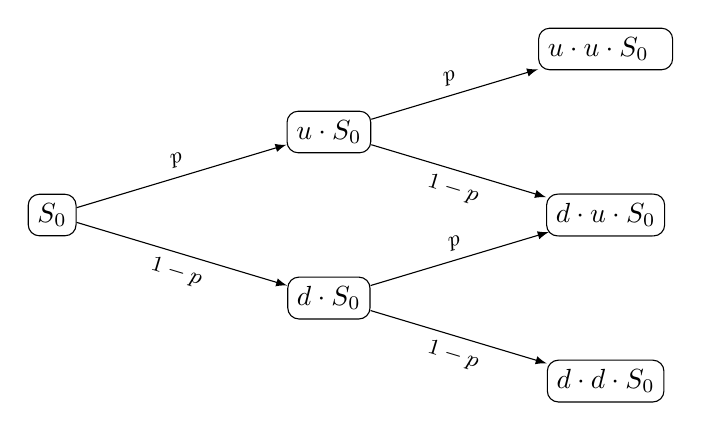
\begin{tikzpicture}
  [
    grow                    = right,
    sibling distance        = 6em,
    level distance          = 10em,
    edge from parent/.style = {draw, -latex},
    every node/.style       = {font=\footnotesize},
    sloped
  ]
  \node [env] {$S_0$}
    child { node [env] {$d \cdot S_0$}
    child { node [env] {$d \cdot d \cdot S_0$}
          edge from parent node [below] {$1 - p$} }
      child { node [env] {$u  \cdot d  S_0$ }
              edge from parent node [above, align=center]{$p$}}
      edge from parent node [below] {$1 - p$} }
    child { node [env] {$u \cdot S_0$}
      child { node [env] {$d \cdot u \cdot S_0$}
          edge from parent node [below] {$1 - p$} }
      child { node [env] {$u \cdot u \cdot S_0$ }
              edge from parent node [above, align=center]{$p$}}
        edge from parent node [above] {$p$} };
\end{tikzpicture}
\end{center}
V vsakem času imamo možnost izbirati med dvema različnima razvojema, kar implicira nedeterministično vedenje. Če preidemo na teorijo algebrajskih učinkov za nedeterminizem, potem v osnovi velja, da jih lahko predstavimo z binarno operacijo \lstinline{izberi} (decide) \cite{introduction}. To je operacija, ki sprejme vrednost tipa \lstinline{unit} in nedeterministično vrne logično vrednost. Za naš primer je to predstavljeno s spodnjo kodo:
\begin{lstlisting}
let obresti  =
	let b = perform (Izberi ()) in
	if b then u else d
;;
\end{lstlisting}
Zgornja funkcija določi obrestno mero tveganega vrednostnega papirja v vsakem naslednjem stanju. Tvegani vrednostni papir bomo v našem modelu imenovali delnica. V skladu z zgoraj opisanim binomskim modelom, lahko izbiramo med obrestnima merama $u$ za dobro in $d$ za slabo stanje ekonomije. Nedeterminizem smo zajeli v operaciji \lstinline{Izberi}. Tipično bi v binomskem modelu ta funkcija delovala verjetnostno. Z neko vnaprej dano verjetnostjo $p$, bi izbrala vrednost \lstinline{true} in z verjetnostjo $1 - p$ vrednost \lstinline{false}. V našem primeru bomo dovolili tudi drugačne definicije.

Prehod trga iz stanja v diskretnem času $t - 1$, v novo stanje v času $t$, določajo obrestne mere vrednostnih papirjev. Zato bomo obresti definirali kot spremenljivo operacijo \lstinline{Obresti}. Spodaj je predstavljena sintaksa za takšno definicijo:
\begin{lstlisting}
type vrednosti_delnic = float list
type obresti = float list
effect Obresti:  vrednosti_delnic -> obresti;;
\end{lstlisting}
Najprej smo za večjo berljivost kode definirali tipa  \lstinline{vrednosti_delnic} in \lstinline{obresti}. Oba sta določena s seznamom  realnih števil. Pri prvem tipu vsako realno število predstavlja vrednost posamezne delnice, pri drugem pa obrestno mero. Število različnih tveganih vrednostnih papirjev na trgu je določeno z dolžino seznama.

V zadnji vrstici zgornje kode nam beseda \lstinline{effect}  pove, da definiramo operacijo, katere delovanje bo predpisoval prestreznik. Za dvopičjem je, kot je značilno za funkcijske programske jezike, naveden tip te operacije. Definirali smo torej novo operacijo, ki vzame stanje vrednosti delnic in nam nedeterministično vrne obrestne mere s katerimi se obrestujejo delnice na prehodu v novo stanje. Definirani operacijo lahko sedaj uporabimo v kodi in z njegovo pomočjo simuliramo preprost primer finančnega trga z vhodnima parametroma:
\begin{itemize}
\item \lstinline{s0} -- vektor začetnih vrednosti delnic v času 0
\item \lstinline{n} -- število obdobij
\end{itemize}
Naša funkcija ne bo popisovala izključno modela Cox-Ross-Rubinstein. Delovanje trga  želimo definirati čim bolj splošno, da bomo kasneje na njem lahko izvajali različne izračune. Seveda bo osnovno delovanje enako kot pri binomskem modelu, le da bo omogočalo tudi realizacije drugih podobnih modelov. Spodaj podajamo predpis funkcije:
\begin{lstlisting}
let obrestuj obresti delnice =
  map2 ( *. ) obresti delnice
;;

let simulacija_trga s0 n =
 (*En korak simulacije*)
  let rec korak k s =
    if k >= n
      then s
    else
      korak (k + 1)  (obrestuj (perform (Obresti s)) s) in
  korak 0 s0
;;
\end{lstlisting}
Simulirani trg vrednostnih papirjev se v vsakem izmed $n$ obdobij obrestuje. V naši kodi smo že lahko uporabljali zgoraj definirano operacijo \lstinline{Obresti}, čeprav še ne vemo kako deluje. Statični tipi v Effu nam zagotavljajo, da se bodo tipi kasneje, ko bomo delovanje operacije \lstinline{Obresti} tudi konkretno določili, ujemali. 

Kakšne bodo obrestne mere delnic bo določal prestreznik, ki ga bomo definirali v nadaljevanju. Prestreznik je tisti del kode, ki pove, kako naj se operacija izvede.

Zaradi enostavnosti v začetku predpostavimo, da imamo en sam vrednostni papir torej, da so vrednosti delnic in obrestne mere predstavljene s seznami dolžine 1. Spodaj definiramo prvi primer prestreznika z imenom \lstinline{deterministicne_obresti}. Deluje tako, da na vsakem prehodu v novo stanje deterministično izbere višjo izmed obrestnih mer $u$ in z njo obrestuje vrednost delnice. Spodaj podajamo kodo:
\begin{lstlisting}
let u = [1.05]
let d = [0.9]

let  deterministicne_obresti = handler
	| v -> v
	| effect (Obresti s) k ->
		continue k  u
;;
\end{lstlisting}
Izraz \lstinline{handler} v zgornji kodi pove, da smo definirali prestreznik. S tem implicira  tip definirane vrednosti in hkrati pove, da   ta sprejme parameter\footnote{Bralec, ki je domač s programiranjem v OCamlu, lahko opazi podobnost med definiranjem funkcije: 

let funkcija = function 

           | x -> ...

Kjer zapis function implicira, da funkcija sprejme nek parameter.} (tipa učinek).

Prvi predpis \lstinline{v -> v} pove da prestreznik, kadar dobi "`čisto"' vrednost (ki ni učinek) vrne kar enako vrednost. Ta predpis je trivialen in ga ni potrebno pisati, zato ga bomo v nadaljevanju izpuščali. Pisali ga bomo le v primerih, ko bomo želeli, da prestreznik spremeni tudi "`čiste"' vrednosti. 

 V drugem primeru predpišemo, da naj prestreznik, kadar v kodi zasledi operacijo \lstinline{Obresti}, njegovo delovanje izvede tako, da vrne obrestno mero $u$ in na ta način izvrši operacijo. 

Parameter \lstinline{k} v zgornjem prestrezniku stoji za kontinuacijo. Zaradi njega se bo izvedel tudi preostanek kode za prestreznikom in bo prestreznik zajel tudi vsak nadaljnji operaciji \lstinline{Obresti} v naši kodi. Sledi da bo v zgornjem primeru v vsakem obdobju prišlo do obrestovanja z obrestno mero $u$. Več o tem kako deluje parameter \lstinline{k} in kakšen je njegov pomen bomo povedali v nadaljevanju. Najprej si poglejmo kako prestreznik uporabimo na zgoraj definirani simulaciji trga:
\begin{lstlisting}
with deterministicne_obresti  handle
	simulacija_trga [20.]  5
;;
\end{lstlisting}
Izračunali smo, koliko po petih obdobjih znaša vrednost vhodnega vrednostnega papirja, ki je imel v času 0 ceno 20. Pri tem je prestreznik \lstinline{deterministicne_obresti}, s katerim smo prestregli celotno funkcijo, določil obrestne mere za obrestovanje v vseh obdobjih. Kadar se je znotraj simulacije trga izvajala npr.\ operacija \lstinline{k + 1} in ostale, ki niso povezane z delovanjem operacije \lstinline{Obresti}, prestreznik nanje ni imel vpliva. Določa le vsako izmed petih obrestovanj v simulaciji. 

Če bi v definiciji prestreznika izpustili parameter za kontinuacijo \lstinline{k}, bi se vrednostni papir kljub petim obdobjem obrestoval samo enkrat, potem pa bi se nadaljevanje prekinilo. Ob klicu zgornje kode bi v tem primeru dobili vrnjeno vrednost $21 = 20 \cdot 1,05$. V našem primeru je torej kontinuacija iz vsebinskih razlogov zaželena, vendar pa to v splošnem ne drži vedno. 

Izjeme, kot eden izmed najpomembnejših učinkov za katere se prestrezniki uporabljajo, po drugi strani nimajo kontinuacije \cite{introduction}. Ko se v kodi sproži izjema, se izvajanje kode prekine,\footnote{Primer izjeme je deljenje z nič. Ko pride do deljenja z 0, se sproži izjema, izvajanje kode pa se prekine, saj rezultata ob deljenju z nič ne moremo dobiti, brez rezultata pa ne moramo nadaljevati računanja.} kar je zaradi napake oz.\ razloga, ki je izjemo sprožil, zaželeno.


Funkcijo \lstinline{simulacija_trga} lahko sedaj preusmerimo z novimi prestrezniki, ki bodo obrestovanje predpisali na drugačen način in s tem realizirali različne modele trga. Poglejmo si še primer prestreznika za obrestovanje, kot ga poznamo iz zgoraj opisanega binomskega modela:
\begin{lstlisting}
let p = 0.6 (*Verjetnost dobrega razvoja ekonomije*)

let binomske_obresti = handler
  | effect (Obresti s) k->
  let izberi = perform (Random_float 1.) < p in
  continue k (if izberi then  u else  d)
;;
\end{lstlisting}
Lokalna spremenljivka \lstinline{izberi} v zgornji funkciji z dano verjetnostjo $p$ pokaže \lstinline{true} in z verjetnostjo $1 - p$ logično vrednost \lstinline{false}. V pogojnem stavku se nato kasneje na podlagi vrednosti funkcije \lstinline{izberi} odločimo, ali se trg obrestuje z obrestno mero $u$ ali $d$. Če simulacijo trga prestrežemo s tem prestreznikom, dobimo eno realizacijo Cox-Ross-Rubinstein modela. Za vhodno začetno ceno delnice $20$ in  za $5$ obdobij, izračun izvedemo z naslednjo kodo:
\begin{lstlisting}
with binomske_obresti handle
	simulacija_trga [20.]  5
;;
\end{lstlisting}


\subsection{Prestreznik za verjetnostno porazdelitev}

V tem podpoglavju bomo z novim prestreznikom spremenili simulacijo trga, ki smo jo definirali zgoraj. Naš cilj je definirati prestreznik, ki ne bo ustrezal zgolj eni realizaciji binomskega modela, temveč bo zajel vsa možna končna stanja ekonomije v tem modelu. Ker je odločitev o tem, v katero stanje bomo prešli, sprejeta na podlagi verjetnosti, ne bomo želeli zgolj množico stanj, temveč njihovo porazdelitev. Tip porazdelitve definiramo kot
\begin{lstlisting}
type porazdelitev = (float * float) list
\end{lstlisting}
torej seznam parov, v katerem bo prvi element para predstavljal vrednost delnice, drugi pa njegovo verjetnost. 

V prestrezniku za porazdelitev želimo ujeti informacije za vse možne razvoje ekonomije skupaj z njihovo verjetnostjo. Spodaj je predstavljena definicija prestreznika za računanje porazdelitve, v kateri je potrebno na smiseln način definirati še funkcijo \lstinline{combine}:
\begin{lstlisting}
let u = [1.05]
let d = [0.9]

let porazdelitev = handler
  | v -> [(v, 1.0)]
  | effect (Obresti s) k -> 
  combine p (continue k u)
		      (continue k d)
;;
\end{lstlisting}
V drugem delu predpišemo, da naj prestreznik operacijo \lstinline{Obresti} izvede tako, da obrestuje na oba možna načina. V kodi zgoraj opazimo predpis \lstinline{continue k u} kot tudi predpis \lstinline{continue k d}. Lahko si predstavljamo, da se na vsakem prehodu iz enega v drugo obdobje računanje razveji v dve veji, tako kot v binomskem drevesu. Dvojna kontinuacija pomeni, da se bo obrestovanje za naslednja obdobja nadaljevalo na obeh vejah. Ko pridemo v zadnje obdobje na koncu vsake veje dobimo vrednost. Vrednosti nato želimo spremeniti v porazdelitve, te pa smiselno združiti med seboj. Potrebujemo torej še predpis, ki bo drevo smiselno združil v eno samo porazdelitev. Želeni proces je za obdobje $n = 2$ in binomski model trga predstavljen s spodnjim drevesom:
\begin{center}
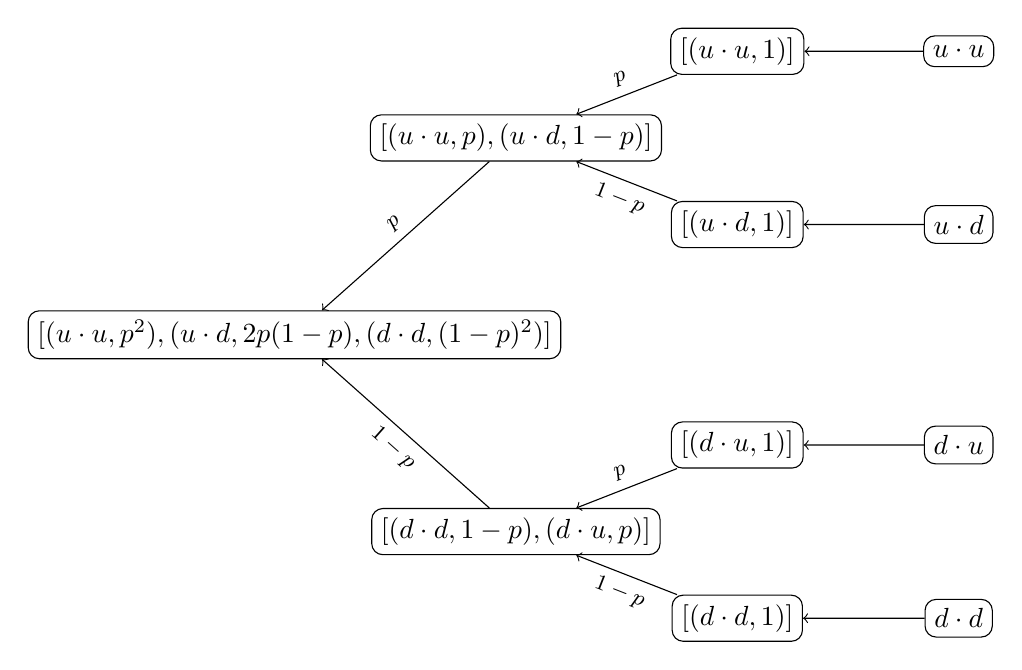
\begin{tikzpicture}
  [
  level distance=1.5cm,
  level 1/.style={sibling distance=5cm},
  level 2/.style={sibling distance=2.2cm},
    grow                    = right,
    sibling distance        = 3em,
    level distance          = 8em,
    edge from parent/.style = {draw, -latex},
    every node/.style       = {font=\footnotesize},
    sloped
  ]
  \node [env] {$[(u \cdot u, p^2),(u \cdot d, 2p(1 - p), (d \cdot d, (1 - p)^2)]$}
    child { node [env] {$[(d \cdot d, 1 - p),(d \cdot u, p)]$}
    child { node [env] {$[(d \cdot d, 1)]$}
    child { node [env] {$d  \cdot d$}
              edge from parent [<-] node [above, align=center]{}}
          edge from parent [<-] node [below] {$1 - p$} }
      child { node [env] {$[(d  \cdot u, 1)]$}
              child {[sibling distance=1mm] node [env] {$d  \cdot u$}
              edge from parent [<-] node [above, align=center]{}}
              edge from parent [<-] node [above, align=center]{$p$}}
      edge from parent [<-] node [below] {$1 - p$} }
    child { node [env] {$[(u \cdot u, p),(u \cdot d,1 - p)]$}
      child { node [env] {$[(u  \cdot d, 1)]$}
      child { node [env] {$u  \cdot d$}
              edge from parent [<-] node [above, align=center]{}}
          edge from parent [<-] node [below] {$1 - p$} }
      child { node [env] {$[(u \cdot u, 1)]$}
      child { node [env] {$u  \cdot u$}
              edge from parent [<-] node [above, align=center]{}}
              edge from parent [<-] node [above, align=center]{$p$}}
        edge from parent [<-] node [above] {$p$} };
\end{tikzpicture}
\end{center}
Prvi vzorec v prestrezniku, ki  "`čiste"' vrednosti \lstinline{v} priredi porazdelitev $[(v, 1.0)]$, naredi prvi potreben korak iz zgornjega drevesa in končne vrednosti v listih drevesa pretvori v porazdelitve. Preostane nam samo še definicija funkcije \lstinline{combine} \cite{examples}, ki bo ustrezno združila dve porazdelitvi, tako kot na zgornji sliki. Poglejmo si predpis ustrezne funkcije:
\begin{lstlisting}
let combine p dist1 dist2 =
  let scale p dist = map (fun (x, q) -> (x, p *. q)) dist 
  in
  let rec add (x, p) = function
    | [] -> [(x, p)]
    | (y, q) :: dist ->
        if x = y then 
	(x, p +. q) :: dist else (y, q) :: add (x, p) dist
    in
    let dist1 = scale p dist1 in
    let dist2 = scale (1.0 -. p) dist2 in
  fold_right add dist1 dist2
;;
\end{lstlisting}
S tako definirano funkcijo \lstinline{combine} zgornji prestreznik smiselno deluje in ga lahko uporabimo na simulaciji trga. Kot rezultat dobimo porazdelitev vrednostnega papirja v končnem obdobju:
\begin{lstlisting}
with porazdelitev handle
    simulacija_trga [20.] 5;;
\end{lstlisting}

\section{Moduli, funktorji in monade}

Alternativa prestreznikom, ki se za podoben način programiranja v funkcijskih programskih jezikih že uporablja, so monade in moduli ter njihova razširitev v funktorje. Uporaba teh je v primerjavi s prestrezniki precej bolj zapletena. Na kratko jih bomo predstavili v nadaljevanju poglavja.

Pogledali si bomo, kako lahko v programskem jeziku OCaml brez uporabe prestreznikov napišemo kodo na nedeterminističen način. Novemu pristopu bo s programiranjem v Eff-u (predstavljeno v prejšnjih poglavjih) skupno to, da bomo kodo napisali  abstraktno oz.\ splošno (simulacija trga bo ostala nespremenjena), na ta način pa bo delovala za več različnih izračunov.

V prvih dveh podpoglavjih si bomo pogledali, kaj so in kako delujejo funktorji in monade, nato pa bomo z njihovo pomočjo izvedli simulacijo binomskega modela. Pri tem si bomo pomagali z identičnimi primeri kot v prejšnjem poglavju, ko smo predstavljali prestreznike v Eff-u. Zaradi enostavnosti bomo ohranjali predpostavko, da imamo na trgu le eno delnico, kljub temu pa bomo računali s seznamom dolžine ena, ki nam bo kasneje omogočil lažjo razširitev v trg z več vrednostnimi papirji.

\subsection{Moduli}

Če v OCamlu želimo daljšo kodo razdeliti na manjše dele (predvsem zapisane v različnih datotekah), jo moramo zapisati v modulih. O modulih lahko razmišljamo kot o zbirki definicij, ki so shranjene v manjših povezanih enotah. Tudi že napisane knjižnice v OCamlu uvozimo v datoteko kot module.

Definirali bomo tip modula z imenom \lstinline{TRG}, ki bo vseboval eno samo funkcijo. To bo funkcija \lstinline{obresti}, ki bo določala obrestne mere in s tem evolucijo trga v vsako naslednje obdobje. Najprej imamo torej definicijo signature oz.\ tipa modula, kot je prikazano spodaj:
\begin{lstlisting}
module type TRG =
sig
  val obresti : vrednosti_delnic -> obresti
end
\end{lstlisting}
Tip modula \lstinline{TRG} opisuje modul, ki vsebuje funkcijo \lstinline{obresti} predpisanega tipa. V modulu tega tipa se lahko nahajajo tudi funkcije, ki jih v signaturi nismo zapisali, vendar ob prevajanju modula, ko se izpiše njegov tip, te funkcije ne bodo vidne. Na ta način bi lahko zunanjemu uporabniku onemogočili uporabo nekaterih funkcij, ki jih modul vsebuje in jih v signaturi ne navedemo, zaradi česar ostajajo skrite.
Kasneje lahko zapišemo več različnih modulov istega tipa. Primerov implementacije tipa modulov \lstinline{TRG} je modul:
\begin{lstlisting}
module Deterministicne_obresti : TRG =
struct
  let u = [1.05]
  let d = [0.9]
  let obresti s = u
;;
end
\end{lstlisting}
V njem, kot je bilo predpisano, najdemo funkcijo \lstinline{obresti}. V tem primeru deluje tako, da vsakega od vrednostnih papirjev obrestuje z višjo izmed obrestnih mer $u$. Da gre za modul tipa \lstinline{TRG}, povemo v prvi vrstici kode za dvopičjem.

Naredimo še en primer modula istega tipa. V njem se obrestne mere izbirajo slučajno, na način, ki je značilen za binomski model trga. Spodaj navajamo opisani modul:
\begin{lstlisting}
module Binomske_obresti : TRG =
struct
  let u = [1.05]
  let d = [0.9]
  let p = 0.6 (*Verjetnost dobrega razvoja ekonomije*)

  let obresti s =
    let izberi = (Random.float 1.) < p in
      if izberi then u else d
;;
end
\end{lstlisting}
Z večimi različnimi moduli torej lahko popišemo različno vedenje nedeterministične operacije \lstinline{obresti}. Opazimo, da se v modulu nahajajo predpisi, ki smo jih v prejšnjem poglavju zapisali v prestreznikih, medtem ko bi signaturo modula lahko primerjali z definicijo nove operacije.

\subsection{Funktorji}

Funktor je modul, ki je parametriziran z drugimi moduli podobo kot je funkcija vrednost, ki je parametrizirana z drugimi vrednostmi (argumenti funkcije) \cite{OCaml}. V njem se bo nahajal del kode, ki bo ostajal nespremenjen. Ker sledimo primeru iz prejšnjega poglavja, bo funktor vseboval funkcijo, ki simulira trg. Spremenljivo operacijo \lstinline{obresti} pa bomo definirali izven funktorja, v vhodnem modulu. 
V spodnji kodi vidimo predpis funktorja, ki kot parameter sprejme modul tipa \lstinline{TRG}:
\begin{lstlisting}
module Simulacija_trga (T : TRG) =
struct
  open T

  let simulacija_trga s0 n=
    let rec korak k s =
      if k >=  n then s
      else
        let s' = 
        List.map2 (fun x y -> x *. y) (obresti s) s in
        korak (k + 1) s'
    in
    korak 0 s0
  ;;

end
\end{lstlisting}
Statični tipi v OCamlu nam omogočajo, da lahko v simulaciji sprožimo operacijo \lstinline{obresti}, še preden je ta definirana. Program pri preverjanju tipov namreč ve, da bo funktor predpis za to funkcijo dobil v modulu, ki ga bo sprejel kot parameter, saj modul tipa \lstinline{TRG} po definiciji vsebuje funkcijo \lstinline{obresti}, katere tip je prav tako znan v naprej in se bo torej preverjeno ujemal z vsemi nadaljnjimi operacijami v funktorju. Sedaj lahko vidimo uporabnost predhodne definicije tipa modula. V njem moramo predpisati vse funkcije, ki jih iz modula želimo prenesti v funktor in jih tam uporabljati.

Kljub temu, da simulacija trga v funktorju ves čas ostaja nespremenjena, lahko z njo delamo različne izračune, odvisno od tega, kako je v vhodnem modulu definirana funkcija \lstinline{obresti}.
Spodaj dodajamo še kodo s katero na zgornjem primeru naredimo izračuna za oba možna predpisa obrestnih mer:
\begin{lstlisting}
module Primer1 = 
       Simulacija_trga (Deterministicne_obresti);;
module Primer2 = Simulacija_trga (Binomske_obresti);;

Primer1.simulacija_trga [20.] 5;;
Primer2.simulacija_trga [20.] 5;;
\end{lstlisting}

\subsection{Monade}

Pri programiranju z moduli in funktorji smo še vedno zelo omejeni, saj funkcija \lstinline{obresti}, ki se nahaja v modulu, lahko vrača le seznam obrestnih mer, ne more pa vračati npr.\ njihove porazdelitve.  Če bi v različnih modulih definirali funkcijo \lstinline{obresti} z različnim tipom, bi namreč prekršili sledeči predpis iz tipa modula \lstinline{obresti : vrednosti_delnic -> obresti}. Če pa bi v tipu modula funkcijo \lstinline{obresti} napisali bolj abstraktno (\lstinline{obresti : vrednosti_delnic -> `a}), tako da bi dovoljevala različne realizacije tipov, bi imeli težave v funktorju. Tam namreč nadaljujemo računanje z obrestnimi merami, ki jih vrne funkcija iz modula. Pri teh računih so uporabljene operacije za sezname realnih števil, ki za drugačne tipe ne bi delovale.

V nadaljevanju bi kodo želeli razširiti tako, da bo funkcija \lstinline{obresti}
lahko vračala tako porazdelitev obrestnih mer, kot tudi eno samo realizacijo, odvisno od tega kaj bomo želeli računati.

V ta namen potrebujemo monade. Monade v OCaml niso neposredno vgrajene, pozna pa jih funkcijski programski jezik Haskell. Napisali bomo modul, ki bo opravljal enako vlogo, kot jo v Haskellu opravljajo monade. 
Monade nam omogočajo, da za vrednosti nekaterih posebnih podatkovnih tipov, kot so podatkovni tipi s kontekstom (z dodano vrednostjo) uporabljamo funkcije za normalne vrednosti in vseeno ohranjamo pomen kontekstov \cite{haskell}. Kaj natančneje to pomeni in kakšna je sintaksa za definiranje monade, bomo preko primerov spoznali v nadaljevanju.

Monada, ki jo bomo napisali za porazdelitev, je v začetku nekoliko zahtevnejša za razumevanje, zato si koncept monad najprej poglejmo na enostavnejšem primeru.


\subsubsection*{Vrednosti tipa Maybe}

Preprost primer monad v Haskell-u so vrednosti tipa \lstinline{Maybe a} \cite{haskell}. Gre za vrednosti, ki predstavljajo vrednosti tipa \lstinline{a}, z možnostjo, da pride do napake in ne dobimo vrednosti tipa
\lstinline{a}. Zato ima tip \lstinline{Maybe} enega izmed dveh možnih predpisov, kot je prikazano v spodnji kodi:
\begin{lstlisting}
type Maybe a = Just a | Nothing
\end{lstlisting}
V tem primeru \lstinline{Nothing} stoji za odsotnost vrednosti tipa \lstinline{a}. Če bi kot rezultat izračuna dobili \lstinline{Nothing}  bi pomenilo, da izračun ni uspel. Predpona \lstinline{Just} pa pomeni, da vrednost tipa \lstinline{a} imamo. Če bi  s pomočjo tipa \lstinline{Maybe} definirali funkcijo deljenje, bi to izgledalo nekako takole:
\begin{lstlisting}
let deli x y =
   match y with
	| 0. -> Nothing
	| y -> Just (x /. y)
;;
\end{lstlisting}
V primeru ko pride do deljenja z nič, bi dobili vrednost \lstinline{Nothing}, v preostalih primerih pa bi se deljenje izvedlo in bi dobili vrnjen rezultat izračuna s predpono \lstinline{Just}. 

Ker monade v programskem jeziku OCaml niso implementirane jih definiramo preko modula. Najprej definiramo njegov tip, v katerem so naštete vse vrednosti, ki jih monada mora vsebovati:
\begin{lstlisting}
module type MONADA =
sig
  type m 'a
  val return : 'a -> m 'a
  val (>>=) : m 'a -> ('a -> m 'b) -> m 'b
end
\end{lstlisting}
Tukaj \lstinline{'a} predstavlja parameter tip, to pomeni, da stoji za poljuben tip, ki pa mora na vseh mestih kjer \lstinline{'a} nastopa, ostajati nespremenjen. Kot vidimo, mora monada vsebovati tri stvari, poglejmo si, kako vsako izmed njih definiramo na primeru monade \lstinline{Maybe}.

Prva stvar, ki jo mora modul tipa \lstinline{MONADA} vsebovati, je konstruktor \lstinline{m}. To je operacija, ki poljubni tip \lstinline{'a} pretvori v novi tip \lstinline{'a m}. Primer konstruktorja je \lstinline{Maybe}.

Kot smo že povedali, monada potrebuje vrednost podatkovnega tipa v kontekstu oz.\ z neko dodano vrednostjo, kar predstavlja črka \lstinline{m} pred parametrom tipa \lstinline{'a}. Za naš primer je ta dodana vrednost tip \lstinline{Maybe}, zato bomo v modulu za prvi predpis napisali:
\begin{lstlisting}
  type m 'a  = Maybe 'a
\end{lstlisting}
Pri definiciji funkcije \lstinline{return} se sprašujemo, kako vrednost tipa \lstinline{'a} smiselno pretvoriti v vrednost tipa \lstinline{m 'a} torej \lstinline{'a} s kontekstom. V našem primeru iz pomena tipa \lstinline{Maybe} sledi naslednji predpis:
\begin{lstlisting}
 let  return x = Just x 
\end{lstlisting}
Če imamo vrednost, potem ji dodamo predpono \lstinline{Just}, ki stoji ravno za prisotnost vrednosti tipa \lstinline{'a}.

Tretja stvar, ki jo še moramo definirati je, kako deluje operacija \lstinline{(>>=)}, ki ji pravimo \lstinline{bind}. V tem delu se sprašujemo, kako ravnati, če imamo vrednost tipa \lstinline{a} s kontekstom \lstinline{'a t} in jo želimo smiselno vstaviti v funkcijo, ki sprejme normalno vrednost tipa \lstinline{`a} in vrne vrednost s kontekstom \cite{haskell}. Poglejmo si, kakšen je predpis v našem primeru:
\begin{lstlisting}
 let (>>=) (Just x) f = f x
 let (>>=) Nothing f = Nothing
\end{lstlisting}
Zanimalo nas je kako vrednost tipa \lstinline{Maybe 'a} smiselno vstavimo v funkcijo tipa \lstinline{('a -> Maybe 'b)}. Ker imamo pri vrednostih tipa \lstinline{Maybe} dva različna možna predpisa, tudi funkcijo \lstinline{bind} definiramo v dveh delih. V primeru, ko imamo vrednost \lstinline{Just x}, funkcijo f  uporabimo na $x$-u, sicer pa vrnemo vrednost \lstinline{Nothing}.
Če sedaj vse naše predpise združimo v skupni modul, dobimo modul tipa \lstinline{MONADA}, ki definira monado \lstinline{Maybe}, kot je prikazano v spodnji kodi:
\begin{lstlisting}
module Mybe_monada : MONADA =
sig
  type m 'a  = Maybe 'a

  let  return x = Just x

  let (>>=) (Just x) f = f x
  let (>>=) Nothing f = Nothing
end
\end{lstlisting}

\subsubsection*{Porazdelitev}

V nadaljevanju želimo definirati modul tipa \lstinline{MONADA}, ki bo obravnaval končne, diskretne porazdelitve. Tip porazdelitve je predpisan z naslednjo kodo: 
\begin{lstlisting}
type finite_dist 'a = ('a * float) list
\end{lstlisting}
Parameter \lstinline{'a} zopet stoji za poljuben tip. V primeru, ko bi imeli porazdelitev vrednosti delnic, bi bil \lstinline{'a} enak tipu \lstinline{float list}, saj so vrednosti delnic z njim predstavljene. Končne porazdelitve tipa \lstinline{'a} predstavljajo naš tip z dodano vrednostjo za katerega bomo napisali monado. Prvo definicijo, ki je v modulu \lstinline{MONADA} potrebna, torej že imamo:
 \begin{lstlisting}
type m 'a  = finite_dist 'a
\end{lstlisting}
Nadalje moramo smiselno napisati predpis funkcije \lstinline{return}, ki vrednosti tipa \lstinline{'a} priredi vrednost tipa \lstinline{finit_dist 'a}.  To bomo storili tako, da bomo vrednost vložili v porazdelitev, v kateri bo kot edina možna izbira izbrana z verjetnostjo 1, to predpisuje naslednja koda:
\begin{lstlisting}
return x = [(x, 1.)]
\end{lstlisting}
Preostane nam še definicija tretjega obveznega predpisa v monadi, operacije \lstinline{>>=}. Sprašujemo se, kako vrednost tipa \lstinline{finit_dist 'a}  smiselno vstavimo v funkcijo, ki sprejme normalno vrednost tipa \lstinline{'a} in vrne porezdelitev tipa \lstinline{finit_dist 'b}.

Če so $a_i$ vrednosti tipa \lstinline{'a} in $p_i, i=1,\cdots,n$ njihove verjetnost, imamo na začetku neko konkretno končno in diskretno porazdelitev:
\[ \left( \begin{array}{cccc}
a_1 & a_2 & \dots & a_n \\
p_1 & p_2 & \dots & p_n  \end{array} \right)\] 

Imamo tudi funkcijo $f$, ki sprejme vrednost tipa \lstinline{'a} in vrne porazdelitev. f lahko kot parameter sprejme katero koli od vrednosti $a_i$. Omenjena preslikava izgleda na sledeči način:
\[ f( a_i) =  \left( \begin{array}{cccc}
b_1 & b_2 & \dots & b_m \\
p_i \cdot q_{i1} & p_i \cdot q_{i2} & \dots & p_i \cdot q_{im} \end{array} \right)\] 
Pri čemer je $f(a_i) = b_1$ z verjetnostjo $q_{i1}$, to verjetnost pa pomnožimo s $p_i$, ki predstavlja verjetnost, da $f$ kot parameter izmed vseh $a$-jev sprejme ravno $a_i$.

Vrnimo se k definiciji funkcije \lstinline{(>>=)}. Zanima nas, kako bi lahko funkcijo $f$ smiselno uporabili na zgornji porazdelitvi $a_i$-jev. To bomo storili tako, da bomo $f$ uporabili na vsakem izmed elementov $a_i$ iz porazdelitve. Pri tem bomo za vsak parameter $a_i$, ki ga bomo vstavili v $f$, kot izhodno vrednost funkcije dobili porazdelitev, kot smo pokazali v zgornjem razmisleku. 

Na koncu bo potrebno še smiselno združiti vse dobljene porazdelitve. S tem problemom smo se že srečali v poglavju s prestrezniki, kjer smo definirali funkcijo \lstinline{combine}. Identično definirano funkcijo uporabimo tudi v tem primeru.

Razmisleku, ki smo ga ravnokar opisali, sledi spodnji predpis funkcije \lstinline{(>>=)}:
 \begin{lstlisting}
 let (>>=) x f =
     combine (List.flatten (List.map (fun (a, p) -> 
      List.map (fun (b, q) -> (b, p *. q)) (f a)) x))
\end{lstlisting}
Če strnemo vse potrebne definicije v skupni modul, dobimo monado za porazdelitev.

\subsection{Simulacija trga z moduli, funktorji in monadami}

Sedaj, ko smo spoznali vsa potrebna orodja, bomo zgoraj napisano kodo združili in preoblikovali tako, da bo tako kot pri prestreznikih, naša simulacija predstavljala model Cox-Ross-Rubinstein. Pri tem bo predpis za simulacijo trga v funktorju ves čas ostajal nespremenjen. Odvisno od definicije vhodnega modula, pa bomo enkrat računali zgolj posamezne realizacije, drugič pa končno porazdelitev modela.

Modul tipa \lstinline{TRG}, ki smo ga definirali zgoraj, razširimo z monado. Operacija \lstinline{obresti} pa ostaja nespremenjena. S tem dobimo sledečo signaturo:
\begin{lstlisting}
module type TRG' =
sig
  include MONADA
  val obresti : 'a  -> m 'a
end
\end{lstlisting}
Nekoliko moramo spremeniti tudi zgornjo simulacijo trga, ki se nahaja v funktorju. Videli smo, da brez uporabe monad ne moremo spreminjati tipov s katerimi računamo v funktorju, zato je morala funkcija \lstinline{obresti} vedno vračati seznam obrestnih mer. Nismo mogli poljubno prehajati na porazdelitve. Spodaj bomo pokazali, kako to omejitev odpravljajo monade. Sedaj namreč funkcije, v katerih smo prej računali z obrestmi, opremimo z operacijo \lstinline{bind} iz monade. Ta bo povedala, kako lahko funkcijo, ki kot parameter sprejme navadne obresti, sedaj  uporabimo tudi na porazdelitvah vseh možnih obrestnih mer na trgu. Porazdelitve namreč predstavljajo dodatni kontekst k tipu obrestnih mer v monadi. Spodaj najdemo popravljeni predpis v funktorju, v katerem ključno vlogo igra funkcija \lstinline{<<=}:
\begin{lstlisting}
module Simulacija_trga' (T : TRG') =
struct
  open T

  let simulacija_trga s0 n =
    let rec korak k s =
      if k >=  n then
        return s
      else
        (obresti s) >>= fun stanje ->
        let s_novi = (List.map2 ( *. ) stanje s) in
        korak (k + 1) s_novi
    in
    korak 0 s0;;

end
\end{lstlisting}
V prvi realizaciji modula želimo računati porazdelitev modela, zato bomo funkcije iz monade predpisali tako, kot  v monadi za porazdelitve. Monadi za porazdelitev smo dodali le funkcijo \lstinline{obresti}, ki vrne celotno porazdelitev obrestnih mer v prihodnjem obdobju in s tem spodaj dobimo prvo realizacijo modula tipa \lstinline{TRG'}:
\begin{lstlisting}
module Obrestuj_porazdelitev : TRG' =
struct
  type m  'a = finite_dist 'a 

  let return x = [(x, 1.)]

  let combine lst =
    let rec add_to dist (a, p) =
      match dist with
      | [] -> [(a,p)]
      | (b,q) :: lst ->
        if a = b
        then (b, p +. q) :: lst
        else (b, q) :: (add_to lst (a, p))
    in
    List.fold_left add_to [] lst

  let (>>=) x f = 
	combine (List.flatten (List.map (fun (a, p) -> 
          List.map (fun (b, q) -> (b, p *. q)) (f a)) x))

  let u = [1.05]
  let d = [0.9]
  let obresti  s = [(u, 0.6), (d, 0.4)]

end
\end{lstlisting}
Če sedaj to monado uporabimo na funktorju, dobimo izračun končne porazdelitve binomskega modela, ki vse vrednostne papirje v dobrem stanju obrestuje z obrestno mero \lstinline{u}, v slabem stanju pa z \lstinline{d}. Spodaj dodajamo še kodo s katero izvedemo izračun:
\begin{lstlisting}
module Primer3 = Simulacija_trga (Obrestuj_porazdelitev);;
Primer3.simulacija_trga [20.] 5;;
\end{lstlisting}
Za primerjavo na drugi strani definiramo še modul za eno samo realizacijo binomskega modela. Tako bomo računali s seznamom obrestnih mer, zaradi česar bo tipa \lstinline{'a} s kontekstom kar enak normalnemu tipu \lstinline{'a}. Tudi definiciji funkcij \lstinline{return} in \lstinline{bind} bosta trivialni, saj bi ta primer lahko definirali že brez uporabe monade. Spodaj kljub temu dodajamo primer kode:
\begin{lstlisting}
module Obrestuj_realizacija =
struct
  type 'a t = 'a

  let return x = x

  let (>>=) x f = f x

  let u = 1.05
  let d = 0.9
  let p = 0.6 (*Verjetnost dobrega razvoja ekonomije*)

  let obresti s =
    let izberi = (Random.float 1.) < p in
    List.map (fun x ->  if izberi then u else d) s
end
\end{lstlisting}

\subsection{Primerjava s prestrezniki}

Identični primer simulacije trga smo zgoraj napisali na z uporabo različnih konceptov na dva različna načina, pri čemer smo sledili želji, da bi funkcija s simulacijo trga ostajala nespremenjena, spreminjale naj bi se le obrestne mere delnic in s tem evolucija simuliranega trga.
Želeli smo, da nam oba načina omogočata tudi spremembo tipa izračuna iz seznama realnih števil v končno porazdelitev seznamov realnih števil (zaradi česar smo morali v drugem načinu vpeljati monade).

V prvem načinu smo uporabili prestreznike in računske učinke, v drugem načinu pa smo potrebovali koncepte modul, funktor in monada, katerih uporaba zahteva nekoliko bolj kompleksen in daljši zapis kode (za isti primer smo napisali dvakrat toliko vrstic kode kot pri uporabi prestreznikov). 

Prednost, ki jo prinašajo prestrezniki je morda še v tem, da je večje število prestreznikov za različne računske učinke med seboj zelo preprosto gnezditi in kombinirati, s čimer se bomo srečali še v nadaljevanju. Videli smo tudi, da prestrezniki lahko sami spremenijo tip izračunov, brez potrebe po definiciji operacije \lstinline{bind}.\footnote{Razlaga skupaj s primerjavo, kako ujemanje tipov zagotavljajo prestrezniki bo poudarjena še v poglavju 6.2 Prestrezniki za operacijo Obrestuj}

Prestrezniki so imeli za svoj nastanek med drugim podlago tudi v monadah, ki so splošnejši koncept in zato lahko pokrivajo več različnih primerov. 





\section{Nedeterministično programiranje in razširitev simulacije trga}

Iz zgornjih primerov že lahko povzamemo nekaj značilnosti, ki jih prinaša nedeterminističen način programiranja in vlogo, ki jo prestrezniki v njem igrajo. Del kode s simulacijo trga smo definirali zgolj enkrat, kasneje je ves čas ostajal nespremenjen. Prestrezniki so nam omogočili, da kljub temu z njim lahko delamo različne izračune. 

V našem primeru je šlo za preproste in krajše kode. Kljub temu si lahko predstavljamo uporabnost takšnega načina programiranja, kjer bi večji del kode lahko ostajal ne spremenjen, z njim pa bi lahko delali različne izračune. Da je to mogoče mora biti jedro kode, ki bo ostalo nespremenjeno, napisano čim bolj splošno, saj bo tako omogočalo več različnih in bolj spremenljivih realizacij trga. Nedeterministične operacije, katerih delovanje želimo spreminjati definiramo kot operacije, ki bodo čakale na predpis iz prestreznika.

V nadaljevanju bo simulacija trga vsebovala večje število spremenljivih operacij, zaradi česar si bomo lahko pogledali, kako enostavno je gnezdenje in kombiniranje različnih prestreznikov, ki bodo predpisovali njihovo delovanje.


Delovanje finančnega trga želimo razširiti tako, da bo poleg tveganih vrednostnih papirjev (delnic) vseboval tudi banko, ki predstavlja ne tvegan, napovedljiv proces. Na finančni trg bomo vključili tudi uporabnika, ki v vsakem obdobju lahko na njem trguje. 
Delnice so sedaj predstavljene s seznamom parov, kjer za vsako delnico najprej navedemo njeno vrednost, nato pa število teh delnic na trgu. Za razširjeni trg najprej definiramo osnovne tipe:
\begin{lstlisting}
type banka = float
type delnice = (float * int) list
type portfelij = int list
type zgodovina = float list
\end{lstlisting}
Portfelij predstavlja seznam celih števil, ki pove, koliko posameznih delnic iz trga imama uporabnik v posesti. Poleg tega bomo v seznam realnih števil včasih morali beležiti zgodovino dogajanja na trgu, da bomo lahko določili želeno trgovalno strategijo. Nadalje definiramo tri nove operacije:
\begin{lstlisting}
effect Trguj : zgodovina * float * delnice -> portfelij;;
effect Obrestuj : delnice -> delnice;;
effect Shrani_zgodovino : zgodovina -> zgodovina;;
\end{lstlisting}
Namesto operacije \lstinline{Obresti} imamo  sedaj operacijo \lstinline{Obrestuj}, ki ne vrača več obrestnih mer, temveč že obrestovane vrednosti delnic. Poleg tega imamo na trgu dodatni nedeterministični operaciji \lstinline{Trguj} in \lstinline{Shrani_zgodovino}, ki sta definirani kot spremenljivi operaciji. Prva izmed njiju določi trgovalno strategijo oziroma portfelij, ki ga uporabnik oblikuje na trgu. Drugi operacija bo v zgodovino shranil podatke o preteklih stanjih finančnega trga, ki bodo potrebni za oblikovanje trgovalne strategije. 

Razširjena simulacija trga sprejme sledeče vhodne parametre:
\begin{itemize}
\item \lstinline{n} -- število korakov simulacije
\item \lstinline{b_p}  -- obrestna mera v banki za pozitivno stanje
\item \lstinline{b_n} -- obrestna mera v banki za negativno stanje
\item \lstinline{b0}  -- začetno stanje na banki
\item \lstinline{s0} --  začetna vrednost trga (vrednosti in števila delnic na trgu)
\item \lstinline{p0}  -- začetni portfelij.
\end{itemize}

\begin{lstlisting}
let simulacija n b_p b_n b0 s0 p0 =
  (* EN KORAK SIMULACIJE *)
  let rec korak k b s zgo p =
   if k >= n then
      let vrednost_p' = vrednost_portfelija p s in
      (b , vrednost_p')
   else
     (* TRGUJEMO *)
     let staraVrednost_p = vrednost_portfelija p s in
     let premozenje = b +. sestej staraVrednost_p in
     let p_novi = 
        perform (Trguj (zgo, premozenje, s)) in
     let p_novi = omeji s  p_novi in
     let novaVrednost_p = vrednost_portfelija p_novi s in
     let b_novo = premozenje -. (sestej novaVrednost_p) in
     (* SHRANI ZGODOVINO *)
     let zgo_nova = 
        perform (Shrani_zgodovino (zgo, s)) in
     (* EVOLUCIJA TRGA *)
     let s_obrestovane = perform (Obrestuj s) in
     let b_obrestovano = 
        b_novo *. (if b_novo < 0.0 then b_n else b_p) in

     korak (k+1) b_obrestovano s_obrestovane 
           zgo_nova p_novi
  in
  korak 0 b0 s0 (cene_delnic s0) p0
  ;;
\end{lstlisting}
Zgoraj napisana funkcija določa splošno delovanje trga. Vedno najprej trguje uporabnik. Izračuna se njegovo premoženje, potem prestreznik pove, kakšen portfelij si oblikuje. Trg portfelij omeji, če je uporabnik želel kupiti več delnic, kot jih trg ponuja. Izračuna se trenutna cena portfelija in se za njeno vrednost zmanjša uporabnikovo stanje na bančnem računu.

Druga operacija nato pove, kateri podatki o trenutnem stanju trga naj se shranijo v zgodovino in prenesejo v naslednje obdobje.
Nazadnje pride še do evolucije trga. Tu se obrestujejo vrednosti delnic, kar določa operacija \lstinline{Obrestuj}, ter bančni račun z eno izmed determinističnih obrestnih mer, odvisno od pozitivnega oz.\ negativnega stanja denarja, ki ga ima uporabnik na bančnem računu.

Simulacijo smo želeli napisati čim bolj splošno, saj je to tisti del kode, ki bo ves čas ostajal nespremenjen. Kljub temu pa bomo na njem izvajali različne izračune in realizacije finančnih modelov. V simulaciji imamo tri nedeterministične operacije, za katere bomo v nadaljevanju napisali različne prestreznike.

\subsection{Prestrezniki za operaciji \lstinline{Trguj} in \lstinline{Shrani_zgodovino}}

 Operaciji \lstinline{Trguj} in \lstinline{Shrani_zgodovino} sta med seboj povezana, saj je trgovalna strategija dostikrat odvisna od tega, kako se je trg razvijal v preteklosti. Prestreznik \lstinline{shrani_zgodovino} bo torej shranil tiste informacije iz preteklosti, ki bodo potrebne za oblikovanje portfelija.

Prestrezniki za operacijo \lstinline{Trguj} bodo v vsakem stanju določili, na kakšen način se oblikuje portfelij. V tem razdelku bomo na začetku imeli oblikovan portfelij, v katerem bodo količine delnic večje od $0$. Potem bomo določili trgovalno strategijo, kot čas ustavljanja\cite{finMath}. To je pravilo, ki v vsakem času pove ali še zadržimo delnico, ki jo imamo ali delnico prodamo. 

Naj cena delnice sledi slučajnemu procesu $(S_t)_{t = 0}^n$. Spodaj si lahko pogledamo dva primera časov ustavljanja za takšno delnico in trgovalno strategijo, ki jo implicirata.

\begin{enumerate}
\item \textbf{Čas prvega padca vrednosti $\tau^1$} je čas ustavljanja in ga lahko definiramo na sledeči način:
\[  \tau^1 =   \left\{ \begin{array}{ll}
         min \{t, S_t < S_{t-1} \}  &, če\{t; S_t < S_{t-1}  \} \neq \emptyset ;\\
         T &, sicer.\end{array} \right. \]      
Delnice bomo v portfeliju držali dokler ne pride do prvega padca njihove vrednosti, nato pa jo bomo prodali. Ker imamo v portfeliju več različnih delnic takšno pravilo velja za vsako posebej. Da bomo vedeli ali je prišlo do padca vrednosti delnice, moramo v vsakem času poznati tudi vrednost iz prejšnjega stanja, zato definiramo prestreznik za operacijo \lstinline{Shrani_zgodovino} na sledeči način:
\begin{lstlisting}
let prejsno_stanje = handler
    | effect (Shrani_zgodovino (zgo, s)) k ->
    (continue k (cene_delnic s))
;;
\end{lstlisting}
Zgornji prestreznik bo v spremenljivko \lstinline{zgodovina} shranil podatke o ceni delnic pred evolucijo trga in jih prenesel v naslednje obdobje. Sedaj lahko definiramo tudi prestreznik za trgovalno strategijo:
\begin{lstlisting}
let drzimo_do_prvega_padca_vrednosti = handler
  | effect (Trguj (zgo, premozenje, s)) k ->
  let cena_s = cene_delnic s in
  let rec cas_ustavlanja zgo cena_delnic =
  match zgo, cena_s with
  | [], [] -> []
  | (x::xs), (y::ys) -> 
  (if x <= y then 1 else 0) :: (cas_ustavlanja xs ys) in

  (continue k (cas_ustavlanja zgo cena_s))
;;
\end{lstlisting}
\item \textbf{Čas prvega povečanja vrednosti za ${}^1/_4 \tau^2$} je prav tako čas ustavljanja. Definiramo ga kot:
\[  \tau^2 =   \left\{ \begin{array}{ll}
         min \{t, S_t > \frac{5}{4}S_0  \}  &, če\{t; S_t > \frac{5}{4}S_0  \} \neq \emptyset ;\\
         T &, sicer.\end{array} \right. \]
\end{enumerate}

V tem primeru je potrebna informacija o cenah delnic v času 0. Oba potrebna prestreznika sta definirana na sledeči način:
\begin{lstlisting}
let zacetno_stanje = handler
    | effect (Shrani_zgodovino (zacetno_st, s)) k ->
    (continue k zacetno_st)
;;

let drzimo_do_povecanja_za_cetrtino = handler
    | effect (Trguj (zgo, premozenje, s)) k ->
    let cena_s = cene_delnic s in
    let rec cas_ustavlanja zgo cena_s =
      match zgo, cena_s with
      | [], [] -> []
      | (x::xs), (y::ys) -> 
      (if (5. /. 4. *. x) >= y then 1 
      else 0) :: (cas_ustavlanja xs ys)
      in
      (continue k (cas_ustavlanja zgo cena_s))
;;
\end{lstlisting}

\subsection{Prestrezniki za operacijo \lstinline{Obrestuj}}

Preostane nam še napisati prestreznik za operacijo \lstinline{Obrestuj}, pri čemer želimo (kot v prejšnjih poglavjih) imeti možnost računanja z več različnimi tipi, npr.\ zgolj z eno samo realizacijo razvojev trga, s končno porazdelitvijo ali pričakovano vrednostjo. Hkrati pa želimo obrestovanje na trgu predpisati s poljubno končno diskretno porazdelitvijo. V ta namen si najprej poglejmo definicijo algoritma, ki izbere naključno vrednost na podlagi dane končne diskretne porazdelitve.

\subsubsection*{Algoritem za generiranje naključnih števil na podlagi končne diskretne porazdelitve}

Najprej definiramo operacijo \lstinline{Izberi}, ki predstavlja Bernoullijevo porazdelitev:
\begin{lstlisting}
effect Izberi : float -> bool;;
\end{lstlisting}
Operacija kot vhodni parameter sprejme realno število (spodaj označeno s \lstinline{p}), ki predstavlja verjetnost s katero je izbrana logična vrednost \lstinline{true} \footnote{Funkcije v tem delu so povzete po \cite{examples} in nekoliko prirejene za naš primer.}, torej ima naslednjo porazdelitev:
\[ Izberi( p) \sim  \left( \begin{array}{cc}
true & false  \\
p & (1 - p)  \end{array} \right)\] 
Na podlagi operacije \lstinline{Izberi} bo sprejeta odločitev, ali iz dane porazdelitve izberemo posamezno vrednost ali ne. Pri tem bo verjetnosti, na podlagi katere bo sprejeta takšna odločitev ustrezala verjetnosti iz dane porazdelitve.

Algoritem bo deloval rekurzivno, robni pogoj pokriva primere v katerih vhodna porazdelitev vsebuje en sam element, tedaj je ta očitno enak izbranemu elementu. V osnovnem koraku rekurzije je z ustrezno verjetnostjo (spodaj \lstinline{normiran_p}) sprejeta odločitev o izbiri prvega elementa, če je le ta izbran se rekurzija konča, sicer v nadaljevanju izbiramo elemente  iz preostanka porazdelitve, torej porazdelitve brez prvega elementa. Opisanemu algoritmu sledi naslednja funkcija:
\begin{lstlisting}
let izberi_iz_porazdelitve l =
  let rec izberi_iz_porazdelitve' acc = function
  | [(x, _)] -> x
  | (x, p)::xs ->
    let normiran_p = (p/.(1. -. acc)) in
    if perform (Izberi normiran_p) then x 
    else 
    	izberi_iz_porazdelitve' (acc +. p) xs
  in
  izberi_iz_porazdelitve' 0. l
;;
\end{lstlisting}
V akumulatorju \lstinline{acc} je shranjena vsota verjetnosti vseh elementov, ki jih v preteklosti nismo izbrali. V zgornji funkciji lahko opazimo, da je verjetnost dana v vhodni porazdelitvi na vsakem koraku normirana z vrednostjo \lstinline{1 - acc}. Poglejmo si idejo dokaza, zakaj tako normirane verjetnosti ustrezajo verjetnostim iz dane porazdelitve. Denimo, da slučajno spremenljivko izbiramo na podlagi spodnje porazdelitve, kjer je $n > 2$:
\[ \left( \begin{array}{cccc}
a_1 & a_2 & \dots & a_n \\
p_1 & p_2 & \dots & p_n  \end{array} \right)\]
Ker je vrednost akumulatorja v začetku enaka 0, je \lstinline{normiran _p} tedaj kar enak $p_1$ in torej velja $P(a_1) = p_1$. Nadalje si poglejmo izračun verjetnosti s katero sta izbrana elementa $a_2$ oz.\ $a_3$:
$$
P(a_2) = (1 - p_1)( \frac{p_2}{1 - p_1}) = p_2 
$$
pri čemer prvi oklepaj predstavlja verjetnost, da ne izberemo prvi elementa iz porazdelitve, ki ga množimo z verjetnostjo, da je izbran drugi element. Vidimo lahko, da se dobljena verjetnost ujema s tisto iz vhodne porazdelitve. Po enakem razmisleku zapišemo še verjetnost izbire tretji elementa iz porazdelitve:
$$
P(a_3) = (1 - p_1) ( 1 - \frac{p_2}{1 - p_1}) ( \frac{p_3}{1 - p_1 - p_2}) = p_3 
$$
Prva dva oklepaja zopet ustrezata verjetnosti, da ne izberemo niti prvega niti drugega elementa v porazdelitvi. V tretjem oklepaju pa se nahaja verjetnost, da je hkrati izbran tretji element. 

S pomočjo podobnega razmisleka, bi lahko pokazali, da se verjetnosti ujemajo za poljuben element iz porazdelitve in torej zgornji algoritem ustrezno deluje. 


Delovanje operacije \lstinline{Izberi} predpišemo s prestrezniki, tako da bo ustrezal binomski porazdelitvi, hkrati pa bo eden izmed prestreznikov vseboval predpis za računanje ene realizacije izračuna, drugi za računanje porazdelitve vseh možnih realizacij, ter tretji za pričakovano upanje. Poglejmo si najprej prvi predpis:
\begin{lstlisting}
let realizacija = handler
  | v -> v
  | effect (Izberi p) k ->
  let izbira = perform (Random_float 1.) < p in
  continue k izbira
;;
\end{lstlisting}
Zgoraj je najprej definiran prestreznik, ki ustreza eni realizaciji izbire, tako da vrne eno izmed logičnih vrednosti \lstinline{true} oz.\ \lstinline{false} z vhodno verjetnostjo $p$ oz.\ $1 - p$.

Nadalje definiramo prestreznik za računanje s porazdelitvami. Predpis sledi razmisleku s katerim smo se že srečali v zgornjih poglavjih. Računanje nadaljujemo za obe logični vrednosti, ter nato končne izračune najprej pretvorimo v porazdelitve, nato pa te porazdelitve smiselno združimo s funkcijo \lstinline{combine}, katere predpis smo tudi že zapisali zgoraj. Poglejmo si opisani prestreznik za porazdelitev:
\begin{lstlisting}
let porazdelitev = handler
  | v -> [(v, 1.0)]
  | effect (Izberi p) k -> 
     combine p (continue k true) (continue k false)
;;
\end{lstlisting}
Pri nedeterminističnem programiranju brez prestreznikov (opisanem v 5. poglavju zgoraj), smo morali uporabiti monade, kadar smo želeli, da identična koda vrača izračune različnih tipov. Torej, kadar npr.\ želimo da so rezultati naših izračunov enkrat zapisani v realnih številih, drugič v seznamih realnih števil, v seznamih parov itd. 

Sedaj, ko smo se že seznanili z delovanjem monad, smo lahko pozorni na to, kako "`zamenjavo tipa"' naredijo prestrezniki. Prestreznik upošteva, da mora operacija \lstinline{Izberi} vračati logično vrednost, da se bo v funkciji \lstinline{ izberi_iz_porazdelitve } ujemal z operacijami, ki s temi vrednostmi računajo naprej. Zaradi kontunuacije \lstinline{k} se računanje nadaljuje, prestrezniki pa nato končnim izračunom spremeni tip v diskretno porazdelitev. 

Prestreznik sam opravi vse potrebne transformacije, brez potrebe po dodajanju bolj kompleksnih konstruktov, kot so monade. \\

Dodajamo še predpis prestreznika za pričakovano vrednost, ki prav tako kot v primeru porazdelitve, računanje nadaljuje za obe logični vrednosti, ko pa pride do končnih izračunov te množi z ustreznimi verjetnostmi ter sešteva med seboj:
\begin{lstlisting}
let rec pomnozi p = function
  | (x, xs) -> 
     (p *. x, (map1 (fun x -> (1.0 -. p) *. x) xs))
;;

let rec zdruzi prvi drugi =
  match prvi, drugi with
  | (x, xs), (y, ys) -> (x +. y, (map2 ( +. ) xs ys))
;;

let pricakovana_vrednost = handler
  | v -> v
  | effect (Izberi p) k ->
  (zdruzi (pomnozi p (continue k true))
  	      (pomnozi (1.0 -. p) (continue k false)))
;;
\end{lstlisting}
Sedaj lahko zgornje funkcije uporabimo za definicijo prestreznika, ki bo delnice obrestoval z naključnimi obrestnimi merami izbranimi glede na končno diskretno porazdelitev. Spodaj podajamo primer v katerem imamo trg s tremi delnicami in tremi možnimi stanji ekonomije:
\begin{lstlisting}
let obrestuj_iz_diskretne_por = handler
  | v -> v
  | effect (Obrestuj s) k ->
    let obresti1 =  [1.2; 0.94; 0.99] in
    let obresti2 = [0.89; 1.1; 1.04] in
    let obresti3 = [0.92; 1.0; 0.87] in
  (continue k (izberi_iz_porazdelitve
     [(obrestuj obresti1 s,0.3);(obrestuj obresti2 s,0.4);
     (obrestuj obresti3 s,0.3)]))
;;
\end{lstlisting}
Imamo torej primer gnezdenih prestreznikov, saj je v predpisu uporabljena funkcija \lstinline{izberi_iz_porazdelitve} v kateri se nahaja operacija \lstinline{Izberi}, zato moramo prestreznik \lstinline{obrestuj_iz_diskretne_por} zajeti še z enim prestreznikom, ki bo določal njeno delovanje. V nasprotnem primeru bi dobili izjemo "`uncaught effect Izberi"'.


Sedaj lahko na simulaciji trga definirani v začetku šestega poglavja, uporabljamo poljubne kombinacije zgoraj definiranih prestreznikov in na ta način izvajamo različne izračune. Spodaj kod primer navajamo eno izmed kombinacij:
\begin{lstlisting}
let primer n =
  with obrestuj_iz_diskretne_por handle
  with drzimo_do_prvega_padca_vrednosti handle
  with prejsno_stanje handle
  simulacija n 1.001 0.9 200.0 
          [(30.0,1); (40.0,1); (50.0,1)] [1; 1; 1]
;;
\end{lstlisting}
Najprej smo simulacijo trga prestregli s tremi prestrezniki, ki ustrezajo definicijam operacij \lstinline{Obrestuj}, \lstinline{Trguj} in \lstinline{Shrani_zgodovino}. Na ta način imamo v primeru določeno trgovalno strategijo in način obrestovanja s katerim trg prehaja v naslednje obdobje.

Potrebujemo še prestreznik za operacijo \lstinline{Izberi}, s katerim bomo za zgornji primer določili ali pri obrestovanju želimo računati s porazdelitvijo, eno verjetnostno realizacijo ali s pričakovano vrednostjo. V spodnji kodi zaporedno izvedemo vse tri izračune:
\begin{lstlisting}
with porazdelitev handle
  primer 3
;;

with realizacija handle
  primer 3
;;

with pricakovana_vrednost handle
  primer 3
;;
\end{lstlisting}
Seveda bi v primeru lahko uporabili drugačno kombinacijo zgoraj definiranih prestreznikov in dobili drugačne izračune. Prav tako bi lahko definirali še nove prestreznike tako, da bi npr.\ iskali trgovalno strategijo, ki optimizira pričakovani dobiček, množico več trgovalnih strategij itd. tako, da možnosti za različne izračune, ki jih odpira primer še zdaleč nismo izčrpali. Vidimo pa, kako lahko na preprost in pregleden način s prestrezniki kombiniramo in gnezdimo več različno delujočih operacije. 

Na tem mestu zaključujemo s primeri simulacije trga, ki so bili tekom celotne diplomske naloge do sedaj med seboj povezani. Tudi v naslednjem poglavju se bomo srečali s simulacijo trga delnic in sicer na podlagi Brownovega gibanja, vendar primer lahko stoji sam zase in ne potrebuje več nobene od dosedanjih definicij.

\section{Prestreznik za spreminjanje stanja in Brownovo gibanje} 

Ogledali smo si že, kako s prestrezniki lahko spreminjamo in preusmerimo izračun kode, vendar imajo ti lahko tudi drugačne vloge. V tem poglavju si bomo najprej na primeru slučajnega sprehoda pogledali uporabo prestreznika za spreminjanje stanj. Pri tem stanje razumemo kot eno možno konfiguracijo pomnilnika ali kot vse (do sedaj) definirane spremenljivke. Stanje bi lahko zajeli tudi širše, kot stanje celotnega računalnika ali celo računalnika skupaj z njegovim uporabnikom. 

Recimo, da imamo stanje, katerega tip označimo z \lstinline{s} in je lahko predstavljeno z realnim številom, urejenim parom ali urejeno n-terico, odvisno od tega koliko spremenljivk želimo imeti. Poleg stanja imamo še dve operaciji, ki spreminjata to stanje v pomnilniku. Operacijo \lstinline{Get: unit -> s} ter operacijo \lstinline{Set: s -> unit} s katerima beremo in nastavljamo stanje.

V ukaznih programskih jezikih (Python, C, C++, Java) programiramo s spremenljivkami, ki hranijo stanje. V teh jezikih pišemo \lstinline{x := e} namesto operacije \lstinline{Set} in preprosto \lstinline{x} namesto \lstinline{Get x}, vendar je to le poenostavljen način pisanja, v ozadju pa sta ti dve operaciji še vedno prisotni. 

Omenjeni operaciji, ki spreminja vrednost spremenljivk v pomnilniku sta učinka. V čistih programskih jezikih (npr.\ Haskell) so namreč funkcije definirane tako, da ne moremo spreminjati nobenega globalnega stanja ali spremenljivke, lahko le delamo izračune in vračamo njihove rezultate \cite{haskell}. Zaradi te lastnosti nam ni treba skrbeti, da bo prišlo do napake, saj v vsakem času točno vemo, kakšna je vrednost posamezne spremenljivke. Ker pa imamo določene primere, ki so neločljivo povezani s spreminjanjem stanj, želimo vseeno imeti tudi to možnost, hkrati pa na drugi strani ohranjati čistost programa. V programskem jeziku Haskell to omogočajo posebne monade za stanja. 

Na kakšen način delujejo monade za stanje v Haskell-u si lahko preberete v 13. poglavju knjige Learn You a Haskell for Great Good! [5]. Tukaj pa si bomo
podrobneje pogledali, koko spreminjanje stanj, torej operaciji \lstinline{Get} in \lstinline{Set}, obvladujejo prestrezniki, pri čemer si
bomo pomagali s primerom slučajnega sprehoda.

\subsection{Prestreznik za stanje in definicija slučajnega sprehoda}

Pri slučajnem sprehodu se v začetku nahajamo v neki vrednosti \lstinline{v_0}, ki bo pri nas predstavljena z realnim številom, nato pa se na vsakem koraku iz te vrednosti naključno premaknemo v neko novo stanje. Novo stanje je torej odvisno od prejšnjega stanja ter prirastka dodanega temu stanju. 

Preden se lotimo definicije slučajnega sprehoda najprej predpišimo dve novi operaciji, s katerima bomo nadzorovali spremembo stanj v slučajnem sprehodu:
 \begin{lstlisting}
 type s = float
 
effect Get: unit -> s
effect Set: s -> unit
\end{lstlisting}
Zaradi boljše preglednosti smo definirali še tip \lstinline{s}, ki je predstavljen z realnim številom in pomeni stanje oz.\ vrednost v kateri se slučajni sprehod nahaja na posameznem koraku. Operacija \lstinline{Set}, katere glavna vloga bo nastavitev novega stanja, nima nobene pomembne vrednosti, ki bi jo morala vrniti, zato vrača samo \lstinline{()}. 

Pri prestrezniku za stanje imamo torej dve operaciji \lstinline{Get} in\lstinline{Set} s prestreznikom spodaj povemo, kako delujeta \footnote{Prestreznik deluje podobno kot monade za stanje v Haskell-u.} \cite{examples}:
 \begin{lstlisting}
let stanje v_0 = handler
  | y -> (fun _ -> y)
  | effect (Get ()) k -> (fun s -> (continue k s) s)
  | effect (Set s') k -> (fun _ -> (continue k ()) s')
  | finally g -> g v_0
;;
\end{lstlisting}
Podani prestreznik je nekoliko bolj zapleten za razumevanje, zato bomo v nadaljevanju za vsakega izmed predpisov v prestrezniku posebej naredili razmislek o tem, kako deluje:
\begin{enumerate}
\item \lstinline{y -> (fun _ -> y)}: \\ Če imamo "`čisto"' vrednost, jo prestreznik pretvori v funkcijo. Ta funkcija bo sprejela nek vhodni parameter, ga zavrgla in vrnila vrednost, ki jo je zajel prestreznik.\footnote{Ta predpis je, če vzporedno gledamo monade za stanje v Haskell-u, podoben definiciji funkcije \lstinline{return}. Omenjena funkcija bi običajno vrednost \lstinline{v} spremenila v izračun stanja, ki vrne enako vrednost \lstinline{v} in nespremenjeno stanje.} 

\item \lstinline{effect (Get ()) k -> (fun s -> (continue k s) s)}: \\ Nadalje imamo operacijo \lstinline{Get}, ki jo prav tako pretvorimo v funkcijo. Predpisana funkcija sprejme trenutno stanje in ga vrne v kontinuacijo \lstinline{k}. Ker funkcija vrne stanje izpoljuje predpis tipa operacije \lstinline{Get}, saj mora ta vrniti stanje. V nadaljevanju bo prestreznik tudi kontinuacijo pretvoril v funkcijo, ki bo naprej računala s stanjem \lstinline{s}. Funkcija pa bo kot parameter potrebovala (še eno) stanje, zato ji ga podamo z dodatnim parametrom \lstinline{s} (zadnji v predpisu).

\item \lstinline{effect (Set s') k -> (fun _ -> (continue k ()) s')}: \\ Parameter \lstinline{s'}, ki ga operacija \lstinline{Set} sprejme, predstavlja novo stanje. \lstinline{Set} spremenimo v funkcijo, ki bo sprejela trenutno stanje, vendar ga ignoriramo, ker ga ne potrebujemo več in nato rečemo kontinuaciji, da je rezultat \lstinline{()}, kar ustreza tipu operacije \lstinline{Set}. V kontinuaciji \lstinline{k} se nato nadaljuje računanje, ki je prav tako zajeto s prestreznikom, kar pomeni, da bo tip izračuna, ki ga bo vrnila kontinuacija, funkcija. To sledi iz predpisa prestreznika, ki "`nečisti"' operaciji in tudi same vrednosti spreminja v funkcije. Ta funkcija bo kot parameter potrebovala stanje, zato ji ga podamo z \lstinline{s'}.

\item \lstinline{finally g -> g v_0}: \\ Prvič se srečamo tudi z zadnjim predpisom v prestrezniku. Videli smo že, da so vsi omenjeni predpisi v prestrezniku vračali funkcije in bodo torej  kodo, ki jo bodo zajeli spremenili v funkcijo. Funkcija pa bo vrnila izračun šele, ko jo bomo klicali na nekem parametru. Zadnji predpis torej pove, naj se na koncu dobljena funkcija, v katero se je pretvorila koda zajeta s prestreznikom, izvede tako, da kot parameter sprejme vrednost \lstinline{v_0}. Iz definicije slučajnega sprehoda v nadaljevanju bo sledilo, da je potreben parameter \lstinline{v_0}, ki predstavlja vrednost v kateri se slučajni sprehod nahaja na začetku.
\end{enumerate}
Sedaj s pomočjo zgornjega prestreznika definiramo slučajni sprehod, v katerem se nahaja tudi operacija \lstinline{Prirastek}, ki bo vračala velikost prirastka na posameznem koraku slučajnega sprehoda in še čaka, da ji prestreznik pove, kako naj deluje. Vhodni parametri napisane funkcije so sledeči:
\begin{itemize}
\item \lstinline{v_0} -- začetna vrednost slučajnega sprehoda
\item \lstinline{n} -- število korakov slučajnega sprehoda
\end{itemize}
Predpis funkcije za slučajni sprefod skupaj z operacijo \lstinline{Prirastek} je sledeč:
 \begin{lstlisting}
effect Prirastek: unit -> float

  let slucajni_sprehod v_0 n =
  with stanje v_0 handle
    (let rec sprehajanje m =
       let novo_stanje =
         perform (Get ()) +. perform (Prirastek ())
       in
       perform (Set novo_stanje);
       if m < n then sprehajanje (m + 1) 
       else perform (Get ())
     in
     sprehajanje 0)
  ;;
\end{lstlisting}
V zgornjem predpisu slučajnega sprehoda je rekurzivna funkcija \lstinline{sprehajanje} že ujeta s prestreznikom za stanja. Funkcija deluje tako, da na vsakem koraku rekurzije najprej vzame stanje, mu prišteje prirastek in vrednost shrani v lokalno spremenljivko \lstinline{novo_stanje}. Nato to stanje sprejme funkcija \lstinline{Set} in ga prenese v naslednji korak. Prestreznik spremembo stanja izvaja tako, da si operaciji \lstinline{Get} in \lstinline{Set} na vsakem koraku (kot parameter, ki ga sprejme funkcija, v katero se operaciji spremenita,) na nek način "`podajata"' spreminjajoče se stanje? \\

Da bomo slučajni sprehod lahko izvedli potrebujemo še prestreznik, ki bo na verjetnosten način predpisal vrednosti prirastkov. Tega bomo v nadaljevanju definirali tako, da bo ustrezal procesu Brownovega gibanja.

\subsection{Prirastki za Brownovo gibanje}

Ime Brownovo gibanje je bilo najprej uporabljeno za pojav kaotično gibanja cvetnega prahu plavajočega v vodi, ki ga je leta 1828 opazoval botanik Robert Brown \cite{brownovoG}. Danes ima več različnih uporabnosti, v fiziki običajno popisuje pojav naključnega gibanja drobnih delcev v tekočini, v matematičnem modeliranju pa z njim generiramo zgornjemu pojavu podobno naključno gibanje. Za nas bo zanimiva predvsem uporaba v ekonomiji, kjer se Brownovo gibanje lahko uporablja pri simulacijah nihanja trga delnic, takšno gibanje vsebuje tudi več  stohastičnih modelov za simuliranje različnih ekonomskih indeksov (kot so Geometrijsko in aritmetično Brownovo gibanje, Ornstein-Uhlenbeckov proces itd.).

Brownovo gibanje je najpreprostejši stohastični proces in ga popisuje Wienerjev proces $W_t$, ki ga karakterizirajo naslednje štiri lastnosti:
\begin{itemize}
 \item $W_0$ = 0
  \item $W_t$ je skoraj gotovo zvezen
  \item $W_t$ ima neodvisne prirastke
  \item prirastki $(W_t - W_s)$, kjer je $0 \leq s \leq t$, so porazdeljeni normalno s povprečjem 0 in varianco $t - s$.
 \end{itemize}
Za naš primer zadostujejo do sedaj povedane lastnosti Brownovega gibanja, pri čemer bomo potrebovali predvsem neodvisnost prirastkov $(W_t - W_s)$ in njihovo porazdelitev. Bralec si lahko podrobnejšo definicijo prebere v knjigi Brownian Motion and Stochastic Calculus \cite{brownovoG}. 

Na Brownovo gibanje lahko gledamo kot na slučajni sprehod z normalno porazdeljenimi prirastki \footnote{Pri tem prirastke ne gledamo v zveznem, temveč v diskretnem času za neko konstantno spremembo časa $dt > 0$}. Za definicijo prirastkov slučajnega sprehoda na način, ki ustreza Brownovem gibanju moramo napisati še algoritem za vzorčenje slučajnih spremenljivk iz normalne porazdelitve, saj je iz prej opisane teorije razvidno, da so tako porazdeljeni prirastki. Kode z opisom tega algoritma tukaj ne bomo dodajali, priložena pa je kot dodatek v datoteki z imenom "`brownovoGibanje.eff"'.

Tukaj bomo privzeli, da v Eff-u že imamo funkcijo \lstinline{gauss e s}, ki vrne eno realizacijo slučajne spremenljivke porezdeljene normalno z pričakovano vrednostjo \lstinline{e} in standardnim odklonom \lstinline{s}.

V spodnji kodi bomo uporabili parametre s sledečim pomenom:
\begin{itemize}
\item \lstinline{v_0} -- začetno stanje delnice oz.\ trenutna vrednost delnice
\item \lstinline{s} -- letni standardni odklon vrednosti delnice od začetne vrednosti
\item \lstinline{dt} -- sprememba časa, kjer je enota leto
\item \lstinline{n} -- število korakov slučajnega sprehoda
\end{itemize}
Najprej definiramo prestreznik za prirastke nato pa z njim prestrežemo funkcijo \lstinline{slucajni_sprehod}, ter jo na ta način spremenimo v Brownovo gibanje:
 \begin{lstlisting}
let normalni_prirastki s dt = handler
  |effect (Prirastek ()) k -> 
     continue k (gauss 0.0 (s *. dt))
;;

let brownianMotion n s dt v_0 =
with normalni_prirastki s dt handle
  slucajni_sprehod v_0 n
  ;;
\end{lstlisting}
Če imamo sedaj npr.\ delnico s trenutno vrednostjo 5 in na preteklih podatkih ocenimo pričakovan letni standardni odklon $3$, lahko simuliramo gibanje vrednosti delnice v prihodnosti z Brownovim gibanjem. Za spremembo časa vzamemo $1/252$, kjer število 252 v imenovalcu predstavlja število delavnih dni v letu. To pomeni, da se bo v simulaciji vrednost delnice spreminjala na vsak delavni dan in bo torej število korakov pomenilo slučajnega sprehoda predstavljalo število delavnih dni.

Spodnja funkcija sprožimo eno realizacijo Brownovega gibanja za navedene parametre in število korakov $25$:
 \begin{lstlisting}
 brownianMotion 25 4.0 (1.0 /. 252.0) 5.0;;
 \end{lstlisting}

Če bi izvedli večje število izračunov z zgornjo funkcijo, bi dobili približen interval na katerem se bo po 25 delovnih dneh domnevno nahaja vrednost delnice. Seveda Gre za napoved vrednosti z Brownovim gibanjem, ki je preprost matematičen model in ima pri napovedovanju svoje omejitve.

\section{Zaključek}

Strnimo še posebnosti ter prednosti programiranja s prestrezniki in algebrajskimi učinki, ki smo ga predstavljali tekom diplomske naloge.

Pri programiranju se pogosto srečujemo s primeri, v katerih lahko podoben postopek oz.\ enak algoritem uporabimo za več različnih izračunov, kar pomeni, da se nam naravno  ponuja nedeterminističen način programiranja. Prestrezniki za algebrajske učinke, ki smo jih uporabljali v programskem jeziku Eff, nam s pisanjem kode, ki deluje zelo splošno, omogočajo lažje in hitrejše programiranje na nedeterminističen način. 

S prestrezniki je spreminjanje delovanja posameznih operacij v kodi enostavno, prav tako je prestreznike za različne računske učinke mogoče pregledno gnezditi in med seboj kombinirati, kar nam omogoča hitro prilagajanje delovanja kode tako, da ta pokriva širok spekter sorodnih primerov. 

S prestrezniki lahko pokrijemo večino primerov za katere se uporabljajo monade, te so sicer nekoliko splošnejše od prestreznikov, vendar pa jih je mnogo težje kombinirati med seboj. Prestrezniki nam ne omogočajo le spreminjanja izračunov kode v druge vrednosti istega tipa, temveč lahko z njimi spreminjamo tudi tipe funkcij, v katerih spremenljive operacije nastopajo. To smo pokazali s primerih zgoraj, kjer smo imeli lahko rezultate izračunov v seznamih realnih števil, v njihovih končnih porazdelitvah, ali pa pričakovanih vrednosti.

Prestrezniki in algebrajski učinki so v programiranju mnogo širši koncept, kot je bil predstavljen v tej diplomski nalogi in se ne uporabljajo le za nedeterministično programiranje ter spreminjanje stanj v transakcijah. Zaradi prednosti, ki jih ponujajo, vzbujajo veliko pozornosti na področju razvoja programskih jezikov. Vedno več je tudi pobud o njihovi implementaciji v že obstoječe programske jezike.


% slovar
\section*{Slovar strokovnih izrazov}

\geslo{algebraic effect}{algebrajski učinek}

\geslo{pure computation}{čisti izračun}

\geslo{stateful computation}{izračun stanja}

\geslo{handler}{prestreznik}

%\pagebreak
%\bibliographystyle{plain}
%% Datoteka za Bibtex
%\bibliography{literatura}

\begin{thebibliography}{1}

\bibitem{algebraic}
Andrej Bauer,
\newblock {What is algebraic about algebraic effects and handlers?}
\newblock {\em ArXiv e-prints}, July 2018.

\bibitem{programming}
Andrej Bauer in Matija Pretnar,
\newblock Programming with algebraic effects and handlers,
\newblock {\em Journal of Logical and Algebraic Methods in Programming},
  84(1):108--123, 2015.

\bibitem{finMath}
K.J. Hastings,
\newblock {\em Introduction to Financial Mathematics},
\newblock Advances in Applied Mathematics. CRC Press, 2015.

\bibitem{brownovoG}
I.~Karatzas, S.~Shreve, S.E. Shreve in S.E. Shreve,
\newblock {\em Brownian Motion and Stochastic Calculus}.
\newblock Graduate Texts in Mathematics. Springer New York, 1991.

\bibitem{haskell}
Miran Lipovaca,
\newblock {\em Learn You a Haskell for Great Good!: A Beginner's Guide}.
\newblock No Starch Press, San Francisco, CA, USA, 1st edition, 2011.

\bibitem{OCaml}
Y.~Minsky,
\newblock {\em Real World Ocaml. Functional Programming for the Masses}.
\newblock Shroff Publishers \& Distr, 2013.

\bibitem{eff}
Matija Pretnar in Andrej Bauer,
\newblock Programski jezik Eff, [ogled 15.~7.~2018], dostopno na \url{https://www.eff-lang.org}.

\bibitem{examples}
Matija Pretnar,
\newblock Eff: examples.
\newblock {\em GitHub repository},
[ogled 15.~7.~2018], dostopno na \url{https://github.com/matijapretnar/eff/blob/master/examples}.


\bibitem{introduction}
Matija Pretnar,
\newblock An introduction to algebraic effects and handlers. invited tutorial
  paper.
\newblock {\em Electronic Notes in Theoretical Computer Science}, 319:19--35,
  2015.

\end{thebibliography}





\end{document}